\documentclass[11pt,a4paper]{article}

\usepackage[margin=2.5cm]{geometry}
\usepackage{graphicx}
\usepackage{booktabs}
\usepackage{float}
\usepackage[hidelinks]{hyperref}

\graphicspath{{../results/}{../img/}}
\setlength{\parskip}{0.5em}
\setlength{\parindent}{0pt}

\title{Neuroscience Assignment: Comparing Audio Models to STG Brain Data with RSA}
\author{Group 10: Ege Postacioglu, Gianluca Privitelli, Nikita Shuvaev, Valentyn Prianikov}
\date{KEN3170 Multi-scale Modeling of Biological Systems}

\begin{document}
\maketitle

%--------------------------------------------------------------------
\section{Introduction}

Computational models of sensory processing can be tested through how accurately they
perform a classification task, and also by comparing internal representations with those
observed in the brain, and how similar they are. In this study, Representational Similarity
Analysis (RSA) was used to compare Artificial Neural Network (ANN) models with neural
responses that were recorded from the Superior Temporal Gyrus (STG), which relates
to acoustic-semantic sound representations. The end goal is to determine what exactly
influences how closely aligned artificial representations are with human brain activity.
The analysis used responses to 288 natural sounds that were divided into 6 different
categories: Animal, music, nature, speech, tools and voice. The 3 models, WaveformModel,
UninspiredModel and InspiredModel have different architectures, training and
layers, so the analysis is contrastive, as the same neural data is used in the models. So
which differences between models correspond to differences in brain alignment?

\begin{table}[H]
\centering
\small
\begin{tabular}{llccc}
\toprule
Model & Input & Convolutional & Recurrent & Nonlinearity \\
\midrule
\texttt{waveform}   & raw waveform & no  & no  & Tanh  \\
\texttt{uninspired} & spectrogram  & yes & no  & Tanh  \\
\texttt{inspired}   & spectrogram  & yes & yes (GRU) & ReLU6 \\
\bottomrule
\end{tabular}
\caption{The three models.}
\end{table}

The models were trained on the ESC-50 dataset (50 sound classes), and their validation accuracy is about 5\%
for \texttt{waveform}, 29\% for \texttt{uninspired} and 39\% for \texttt{inspired}. We also compare them to
YAMNet, a larger pretrained audio model. We did not do the bonus Part II.

%--------------------------------------------------------------------
\section{Methods}

We used our own RSA toolbox from the practical. For every system we made a $288 \times 288$ RDM:
\begin{itemize}
  \item the STG brain data,
  \item every layer of the three models untrained (5 random seeds each),
  \item every layer of the three models trained (the 5 given checkpoints each),
  \item every layer of YAMNet.
\end{itemize}
The layer activations were taken with \texttt{extract\_activations} and flattened into one vector per sound.
We made the RDMs with two distance measures: Euclidean distance and correlation distance ($1 - r$).

To compare a model to the brain, we correlated the upper triangle of the model RDM with the upper triangle of
the brain RDM. We used Pearson for the Euclidean RDMs and Spearman for the correlation RDMs. The resulting
$r$ is the brain alignment.

\textbf{Statistics.} There are 5 copies of each model type, so for every layer we report the mean $r$ over
the 5 runs with a 95\% confidence interval (mean $\pm$ 1.96 $\cdot$ SEM). To check if two groups are really
different, we used a Welch $t$-test on the 5 values of each group. YAMNet is only one model, so it has no
confidence interval.

For the t-SNE plots we ran t-SNE on each layer and on the brain data and coloured the points by category. To
compare the plots, we counted how often a sound's nearest neighbour on the plot has the same category
(chance is 17\%).

%--------------------------------------------------------------------
\section{Results}

All alignment values are low (the highest is about 0.12), which is expected with data from one participant.
So we mainly compare the models with each other. The results below use Euclidean RDMs with Pearson.

\begin{table}[H]
\centering
\small
\begin{tabular}{llll}
\toprule
Model & Condition & Best layer & $r$ (95\% CI) \\
\midrule
\texttt{waveform}   & untrained & classifier & $-0.008 \pm 0.021$ \\
\texttt{waveform}   & trained   & classifier & $0.015 \pm 0.017$ \\
\texttt{uninspired} & untrained & conv 2     & $0.099 \pm 0.013$ \\
\texttt{uninspired} & trained   & conv 1     & $0.101 \pm 0.009$ \\
\texttt{inspired}   & untrained & conv 2     & $0.065 \pm 0.031$ \\
\texttt{inspired}   & trained   & conv 1     & $0.113 \pm 0.007$ \\
YAMNet              & pretrained & layer 7   & $0.115$ \\
\bottomrule
\end{tabular}
\caption{Best layer of each model.}
\end{table}

\begin{table}[H]
\centering
\small
\begin{tabular}{lccc}
\toprule
Comparison & $r_1$ & $r_2$ & $p$ \\
\midrule
\texttt{inspired} conv 1, trained vs untrained       & 0.113 & 0.056 & 0.003 \\
\texttt{uninspired} classifier, trained vs untrained & $-0.037$ & 0.062 & $<0.001$ \\
\texttt{uninspired} vs \texttt{waveform} (trained, best layer) & 0.101 & 0.015 & $<0.001$ \\
\texttt{inspired} vs \texttt{uninspired} (trained, best layer) & 0.113 & 0.101 & 0.08 \\
\bottomrule
\end{tabular}
\caption{Main Welch $t$-tests (5 runs per group).}
\end{table}

\textbf{Training (Figure~\ref{fig:training}).} Training improves the conv layers of \texttt{inspired} (conv 1
goes from 0.056 to 0.113). For \texttt{uninspired} the conv layers stay about the same. The higher layers (fc,
rnn and classifier) get worse after training and end up around zero or below. \texttt{waveform} stays around or
below zero.

\begin{figure}[H]
\centering
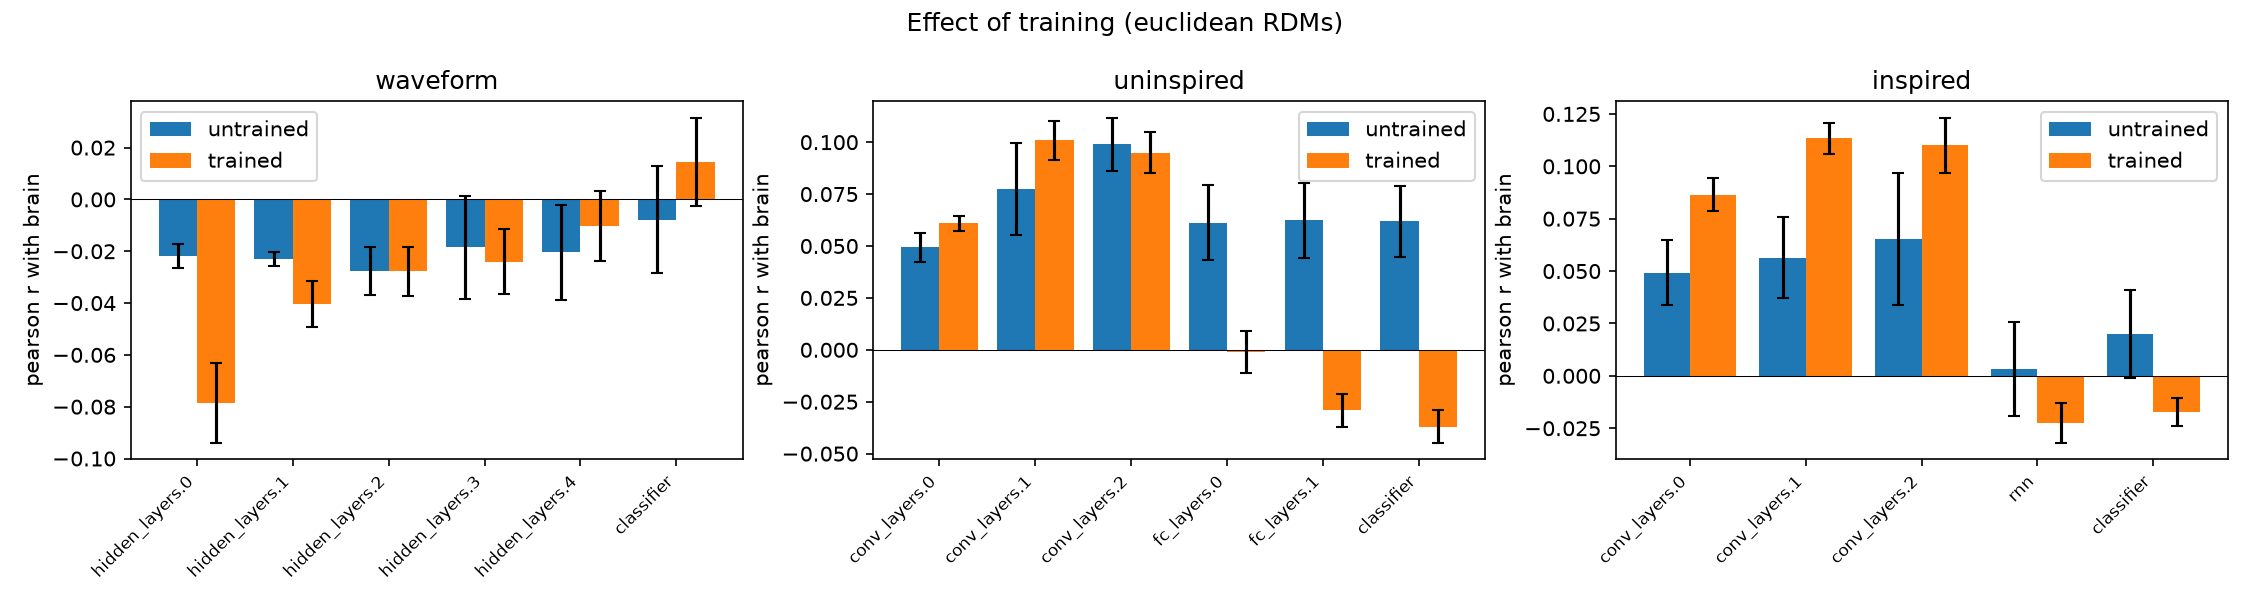
\includegraphics[width=\textwidth]{training_euclidean_pearson.png}
\caption{Untrained vs trained models per layer (mean and 95\% CI).}
\label{fig:training}
\end{figure}

\textbf{Architecture (Figure~\ref{fig:architecture}).} The two spectrogram models align much better than
\texttt{waveform}. \texttt{inspired} is only a little better than \texttt{uninspired}, and the difference is not
significant ($p = 0.08$). Both are close to the best YAMNet layer.

\begin{figure}[H]
\centering
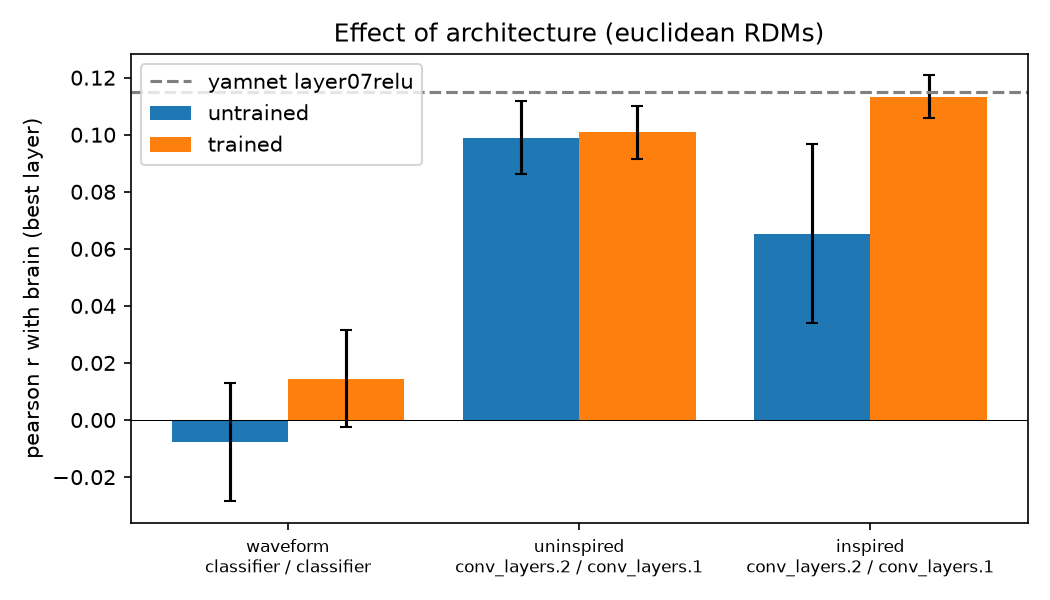
\includegraphics[width=0.7\textwidth]{architecture_euclidean_pearson.png}
\caption{Each model at its best layer. The dashed line is the best YAMNet layer.}
\label{fig:architecture}
\end{figure}

\textbf{Depth (Figure~\ref{fig:depth}).} In the trained conv models the middle conv layers align best, and the last
layers align worst. YAMNet shows the same pattern: it is highest around layer 7 and drops to around zero or below in
the last layers.

\begin{figure}[H]
\centering
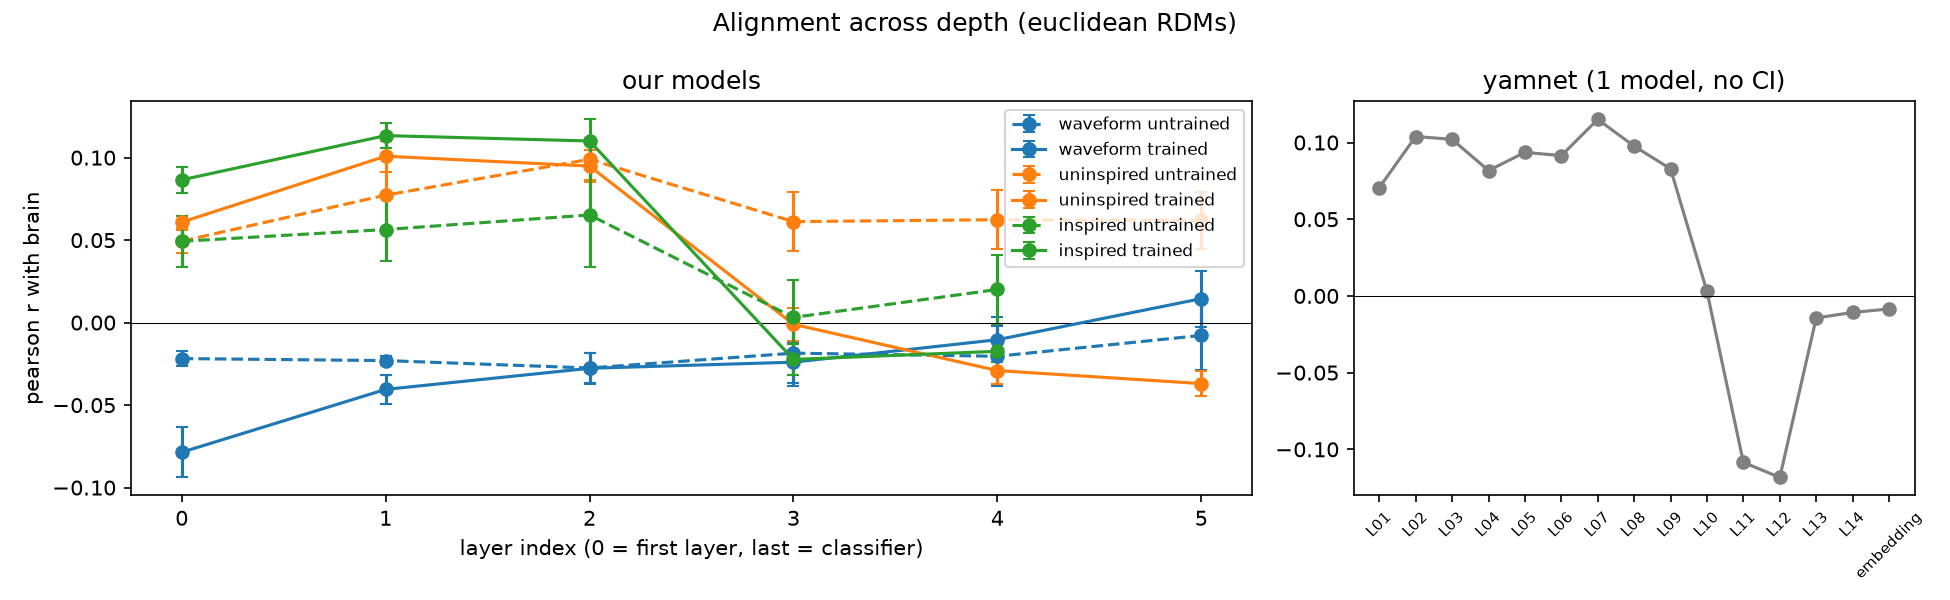
\includegraphics[width=\textwidth]{depth_euclidean_pearson.png}
\caption{Alignment across the layers (left: our models, right: YAMNet).}
\label{fig:depth}
\end{figure}

\textbf{RDMs (Figure~\ref{fig:rdms}).} The brain RDM shows some category structure, but not six clear blocks:
animal and music are close together. The trained conv models and YAMNet show clear category blocks, while
\texttt{waveform} shows none. With correlation RDMs and Spearman all values are lower (below 0.1) and the order
of the layers changes a bit, but \texttt{waveform} is still the worst.

\begin{figure}[H]
\centering
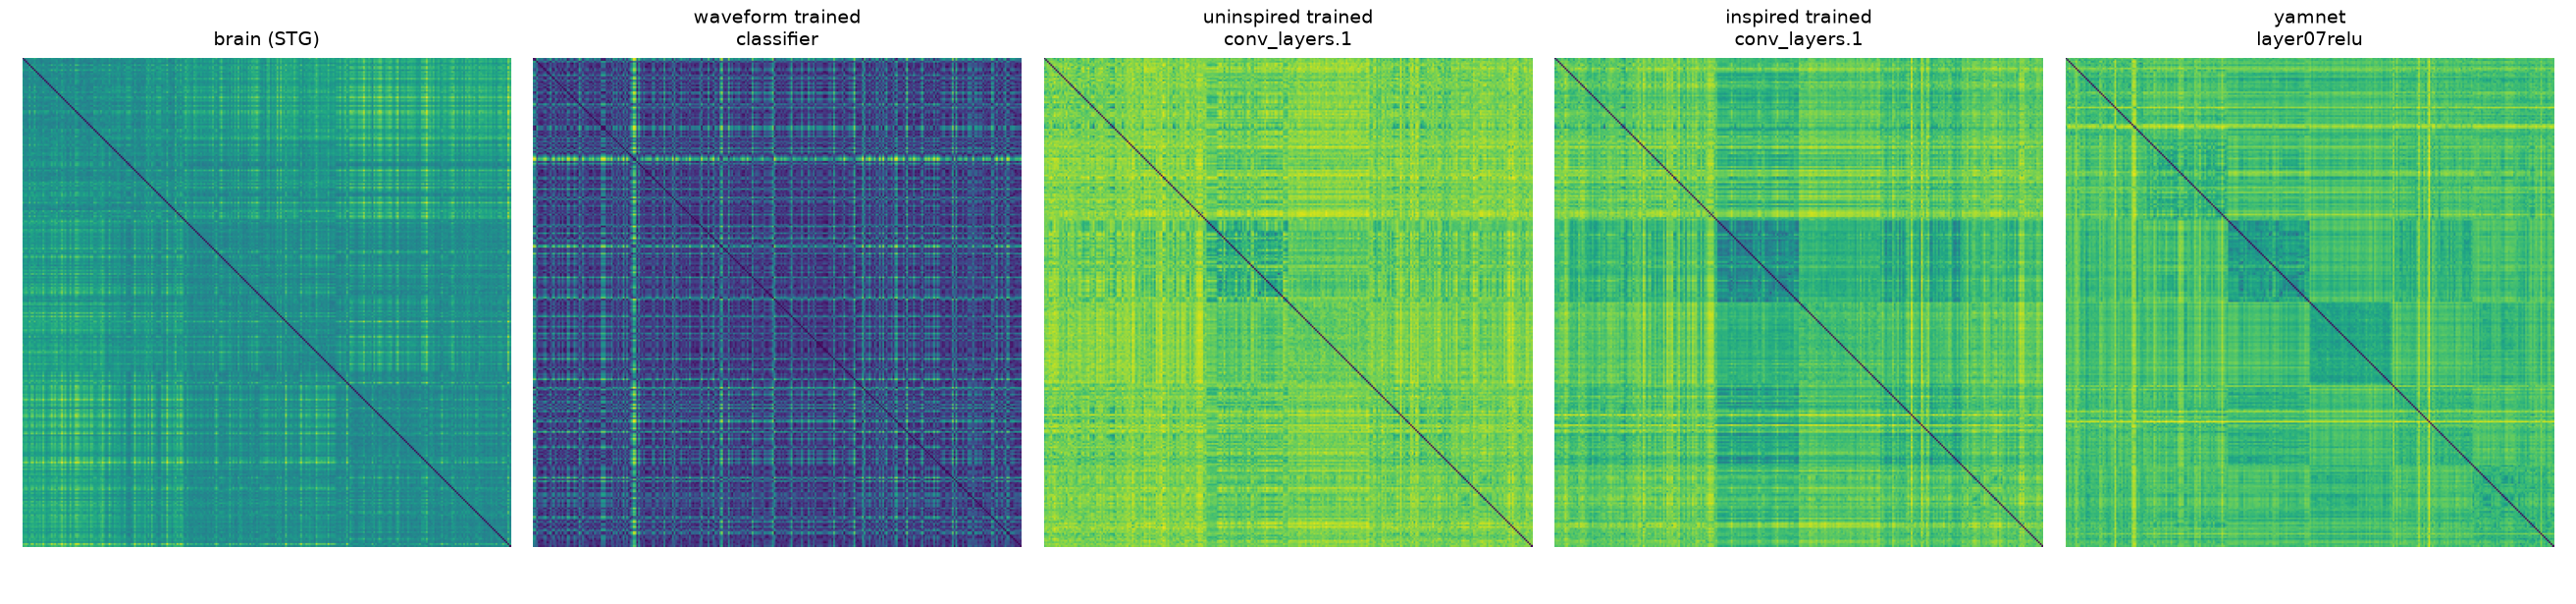
\includegraphics[width=\textwidth]{rdms_euclidean_pearson.png}
\caption{Brain RDM and the best layer of each trained model and YAMNet.}
\label{fig:rdms}
\end{figure}

\textbf{t-SNE (Figures~\ref{fig:tsne_brain} and \ref{fig:tsne_inspired}).} In the brain plot, animal and music
form one cluster and the rest is mixed (49\% same-category neighbours). YAMNet separates the categories much
better (79\%). \texttt{waveform} is at chance on every layer (about 20\%). In the trained conv models, conv 2 is
the most separated (59\% \texttt{uninspired}, 65\% \texttt{inspired}).

\begin{figure}[H]
\centering
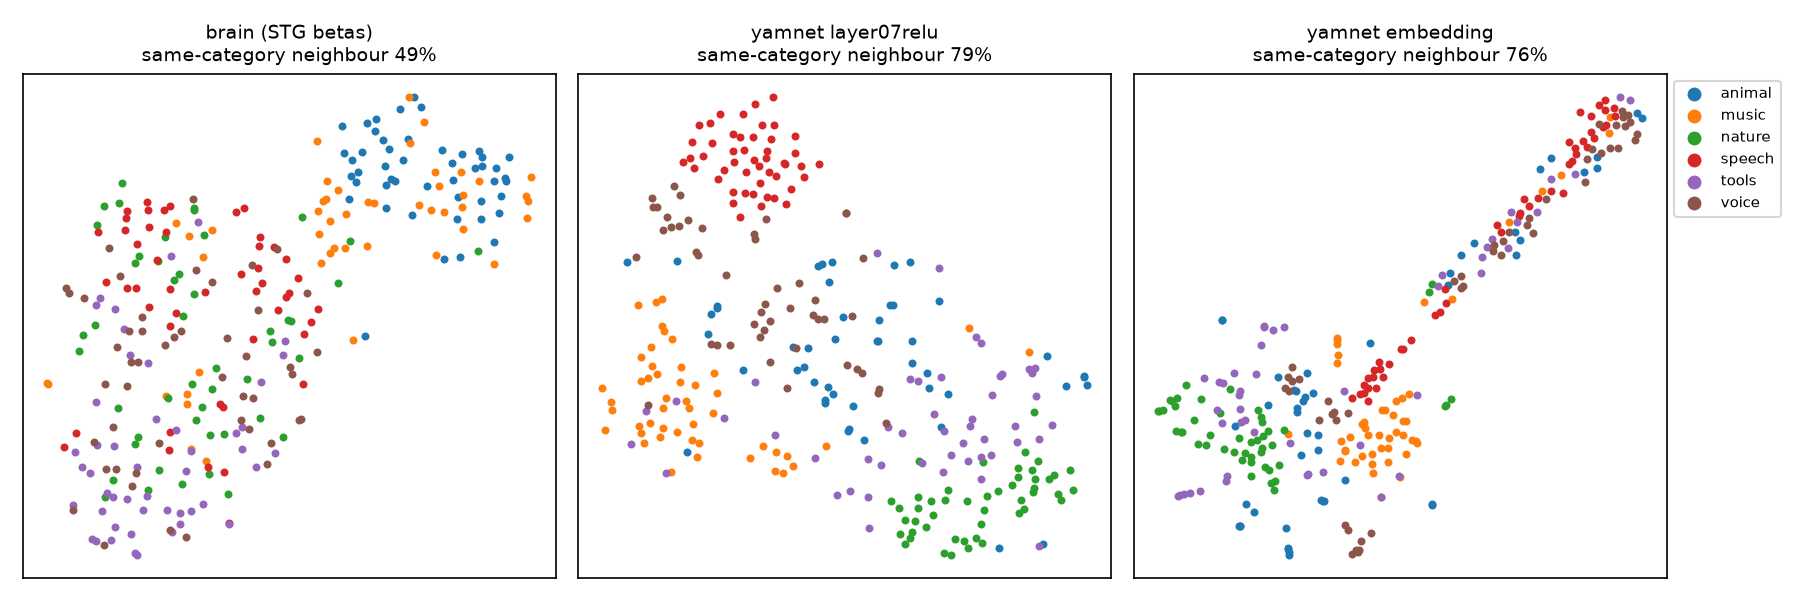
\includegraphics[width=\textwidth]{tsne_brain_yamnet.png}
\caption{t-SNE of the brain data and two YAMNet layers.}
\label{fig:tsne_brain}
\end{figure}

\begin{figure}[H]
\centering
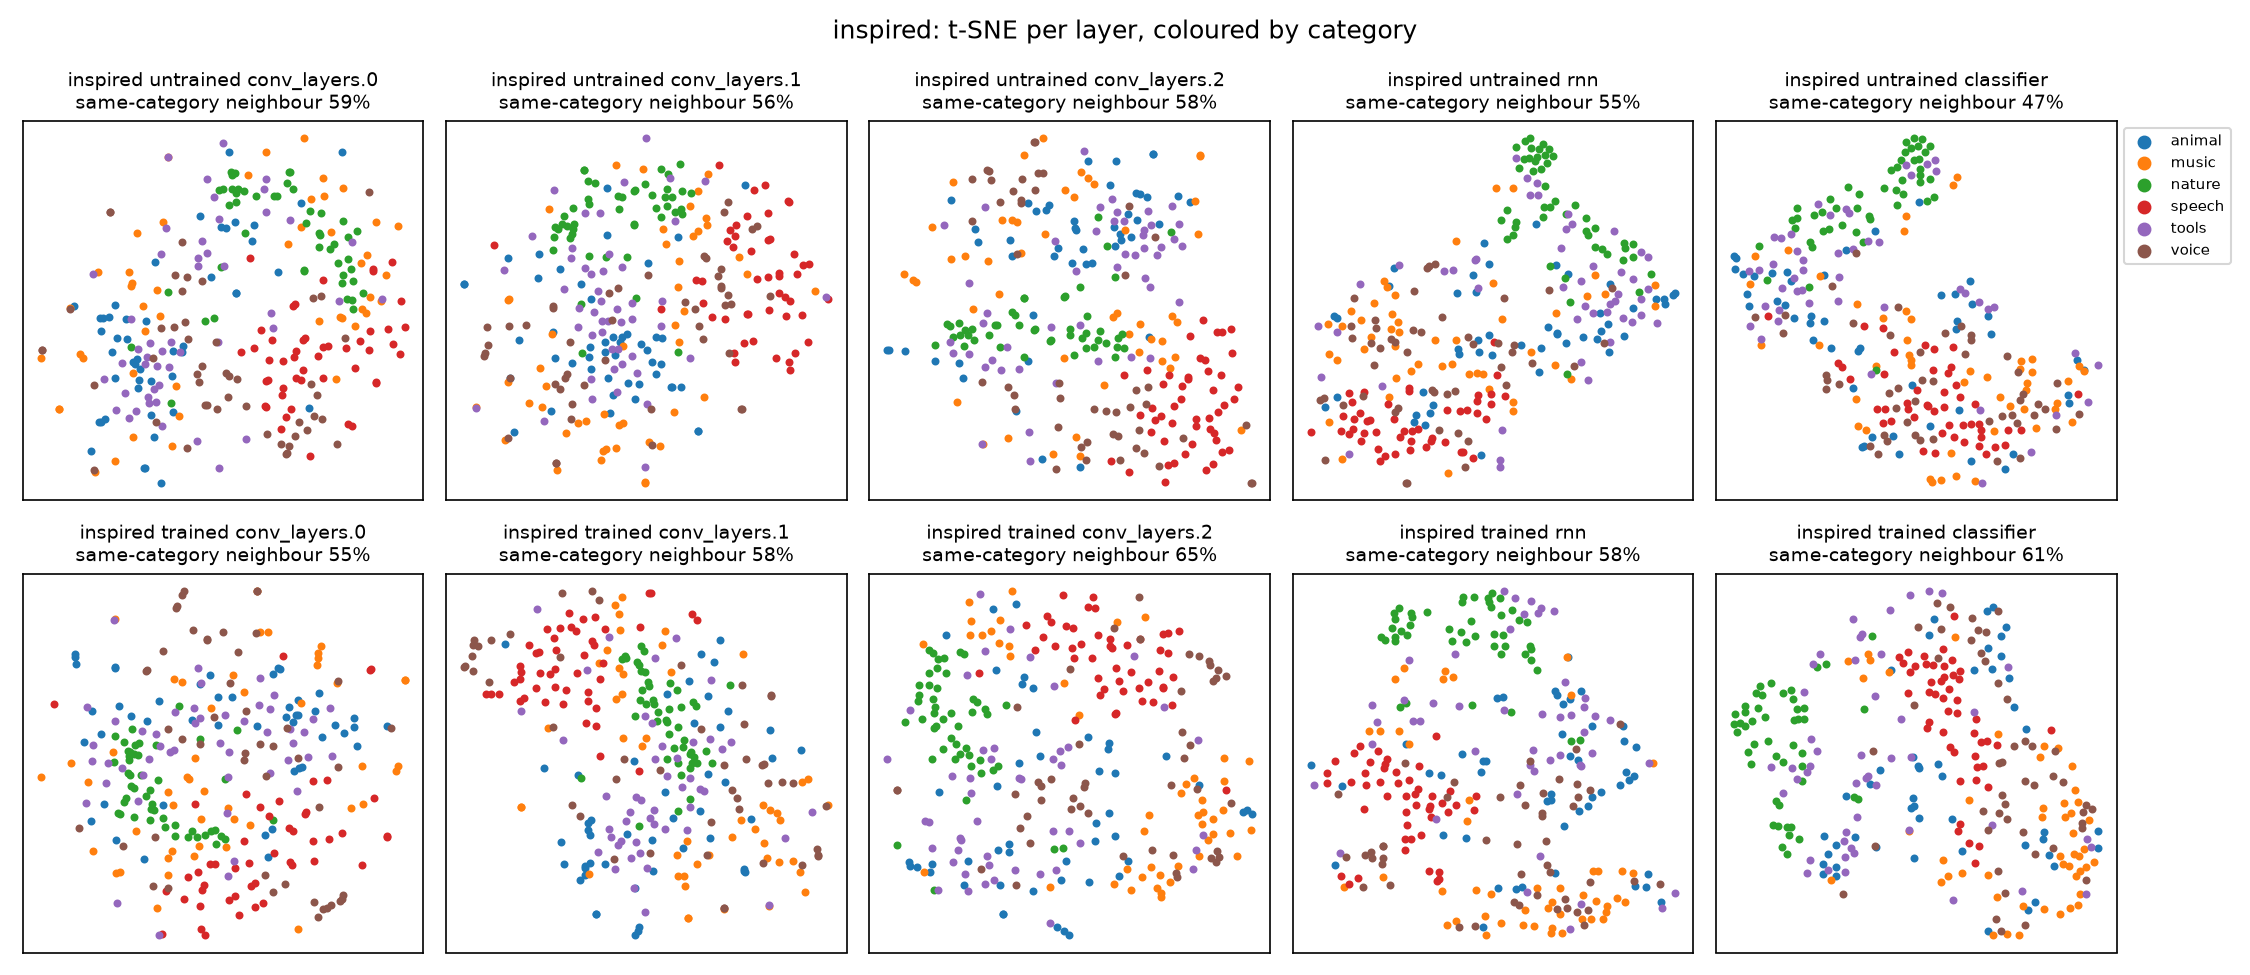
\includegraphics[width=\textwidth]{tsne_inspired.png}
\caption{t-SNE of every layer of \texttt{inspired}, untrained (top) and trained (bottom).}
\label{fig:tsne_inspired}
\end{figure}

%--------------------------------------------------------------------
\section{Discussion}

\textbf{Untrained vs trained.} The untrained conv models already match the brain quite well, so a big part of
the alignment comes from the architecture and the spectrogram input, not from training. Training helps the conv
layers of \texttt{inspired}, but it makes the top layers worse. We think this is because training on the 50
ESC-50 classes makes the top layers very specific to that task, and the STG does not work like that.
\texttt{waveform} never really learned the task, so training did not help it.

\textbf{Models against each other.} The biggest improvement is going from the raw waveform to a spectrogram
with convolutions, so the type of input matters a lot. Adding the GRU did not clearly help, and the GRU layer
itself does not match the brain. \texttt{inspired} also uses ReLU6 and trains better, so we cannot say which of
these changes causes its small advantage.

\textbf{Depth.} The middle layers match the STG best in the conv models and in YAMNet. This fits the idea
that the STG is an in-between step from sound to meaning: the first layers are too close to the raw sound and
the last layers are too close to the class labels.

\textbf{t-SNE.} The t-SNE plots show that separating the categories well is not the same as matching the
brain. YAMNet separates the categories better than the brain does, but it aligns only about as well as our
best conv layers. The layers that match the brain best are only partly organised by category, just like the
STG.

%--------------------------------------------------------------------
\section{Future work}

To make the models more like the brain, we could add more details from the auditory pathway:
\begin{itemize}
  \item Build the model in stages that follow the pathway from the ear to the STG (brainstem, thalamus,
  primary auditory cortex, STG), with one block per stage.
  \item Keep the frequency order (tonotopy) through the convolutional layers.
  \item Add recurrence inside each stage and feedback connections from higher to lower stages, since the
  cortex has many feedback connections.
  \item Use ReLU or ReLU6 everywhere, because neurons cannot fire negatively.
\end{itemize}
Other things that could help are pretraining on a larger dataset before training on ESC-50, and using brain
data from more participants.

\end{document}
